\setcounter{chapter}{3}
\setcounter{section}{0}
\part{MÉTODOLOGÍA DE LA INVESTIGACIÓN} 

\section{Localización}

El proyecto se realizó en la Universidad Técnica Estatal de Quevedo (UTEQ), campus "La María", ubicada en el Cantón Quevedo de la Provincia Los Ríos, en Ecuador. Previo a la obtención del título de Ingeniero en Sistemas. La ejecución del proyecto duró 4 meses, desde el mes de junio de 2022 hasta el mes de septiembre del 2022.

\begin{figure}[h!]
	\caption{Localización de la UTEQ campus "La María".}
	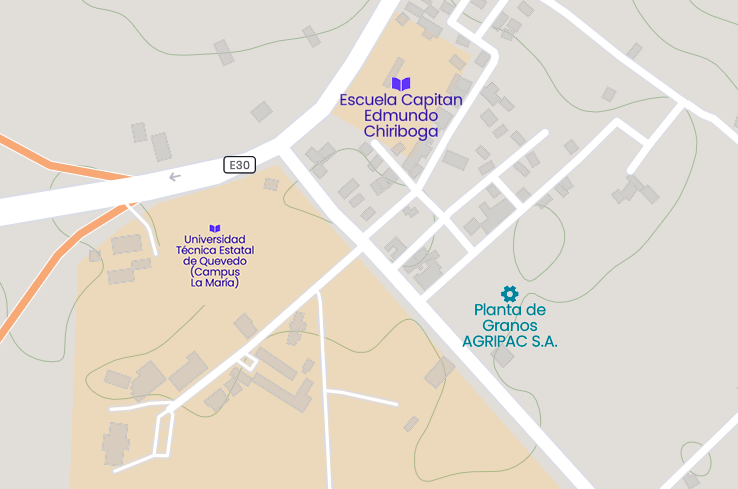
\includegraphics[width=12cm]{img/campuslamaria.png}
	\label{fig:lamaria}
	\textbf{\\ ELABORADO: DÚVAL CARVAJAL SUÁREZ}
\end{figure}.

\section{Tipo de investigación}

\subsection{Investigación aplicada}

La ejecución de este proyecto implico realizar una investigación de tipo aplicada. Se analizarán conceptos como lo que son los compiladores, lenguajes de modelado UML y detección de errores. El trabajo presentado fue un proyecto de desarrollo, es decir que se aplicaron los conceptos investigados al producto final para que cumpla con todo lo establecido en apartado inicial de este trabajo.

\section{Método de investigación}

\subsection{Método inductivo}

Con la ayuda del método inductivo se pudo conocer que para los desarrolladores de software es necesario contar con algún tipo de conocimiento sobre lenguajes de modelado, llevar aun orden de trabajo mediante una metodología de desarrollo ágil que permita satisfacer las necesidades y requisitos que fueron planteados por el cliente.

\subsection{Método deductivo}

El método deductivo permitió emplear de la problemática del proyecto presentado, el cual se evidencio la manera de cómo obtener un diagrama de clases de forma automática mediante las descripciones de los casos de uso. Además de potenciar el uso de la herramienta TDDT4IoTS. El objetivo de esta librería es disminuir el tiempo que le toma a un desarrollador empezar con el modelado un sistema informático empezando por la generación del diagrama de clases.

\subsection{Método analítico}

Se empleo el método analítico para extraer los símbolos que serán analizados por la librería, con el objetivo de conocer que símbolos serán los que se lograrán identificar en las descripciones de los casos de uso. En este caso se debe conocer exactamente los datos de entrada para ser procesados y generar lo requerido por el proyecto presentado.

\section{Fuentes de recopilación de información}

\subsection{Fuentes primarias}

Entre las fuentes primarias que se recurrió para el desarrollo de la librería JavaScript que permitirá detectar los errores de escritura de los casos de uso escritos en un lenguaje de símbolos , la información y la metodología de desarrollo se acoplo a los conceptos del manifiesto ágil, generando una metodología adapta a las necesidades del proyecto tomando en cuenta los 12 principios del desarrollo de software ágil.

\subsection{Fuentes secundarias}

Como fuente secundaria para el soporte del desarrollo de la librería JavaScript se puede mencionar que toda la información fue recopilada mediante el uso de Internet, artículos científicos, libros y folletos.

\section{Diseño de la investigación}

Para el desarrollo del presente proyecto se tomarán en cuenta la ejecución de varias etapas, aplicando el Modelo de Prototipado para desarrollar un prototipo de la aplicación web que utilice el producto final de esta investigación. A continuación, se describe el enfoque metodológico correspondiente a cada una de las fases. 

\subsection{Metodología de desarrollo aplicada al proyecto}

Para ejecutar el proyecto presentado, se analizó el Manifiesto por el Desarrollo Ágil de Software. La metodología aplicada a este proyecto se basó los Principios del Manifiesto Ágil. Con el objetivo de cumplir las directrices de una metodología ágil. En la tabla \ref{tab:analisis_principios} se redactan los 12 principios del manifiesto ágil y análisis aplicado a la metodología \cite{managil}.

\begin{table}[h!]
	\caption{Los 12 principios ágiles y su análisis en la metodología.}
	\label{tab:analisis_principios}
	\begin{tabular}{p{7cm}p{7cm}}
		\toprule
		\textbf{Principios del manifiesto ági}l & \textbf{Análisis aplicado a la metodología} \\
		\midrule
		\textit{1. Nuestra mayor prioridad es satisfacer al cliente mediante la entrega temprana y continua de software con valor}  & Para la entrega continua de cambios sobre el desarrollo del guion, se describieron varias fases de desarrollo. \\
		\addlinespace
		\textit{2. Aceptamos que los requisitos cambien, incluso en etapas tardías del desarrollo. Los procesos Ágiles aprovechan el cambio para proporcionar ventaja competición al cliente.}   & A lo largo de la ejecución de la metodología se podrá realizar modificaciones en los requisitos que se plantearon, con el objetivo de mejorar las funcionalidades del software. \\
		\addlinespace
		\textit{3. Entregamos software funcional frecuentemente, entre dos semanas y dos meses, con preferencia al periodo de tiempo más corto posible.}   & Se organiza una fase en la que se genera todo el código fuente del sistema informático con comprobaciones constantes. \\
		\addlinespace
		\textit{4. Los responsables de negocio y los desarrolladores trabajamos juntos de forma cotidiana durante todo el proyecto.}   & Durante la ejecución del proyecto se mantiene constante contacto con el cliente \\
		\addlinespace
		\textit{5. Los proyectos se desarrollan en torno a individuos motivados. Hay que darles el entorno y el apoyo que necesitan, y confiarles la ejecución del trabajo.}   & Para brindar el entorno de trabajo adecuado a los desarrolladores, la metodología se la puede llevar a cada de forma remota, es decir en la comodidad de su hogar. \\
		\addlinespace
		\textit{6. El método más eficiente y efectivo de comunicar información al equipo de desarrollo y entre sus miembros es la conversación cara a cara.}  & Se realizaron reuniones virtuales y en ciertas ocasiones reuniones presenciales con el cliente final. \\
		\addlinespace
		\textit{7. El software funcionando es la medida principal de progreso.}  & Se realiza el desarrollo completo de cada módulo que fue designado. \\
		\addlinespace
		\textit{8. Los procesos Ágiles promueven el desarrollo sostenible. Los promotores, desarrolladores y usuarios debemos ser capaces de mantener un ritmo constante de forma indefinida.}  & Dentro de la metodología se especifican varias fases en las cuales todos los integrante pueden opinar o tratar con mejoras mediante ideas claras y precisas. \\
		\addlinespace
		\textit{9. La atención continua a la excelencia técnica y al buen diseño mejora la Agilidad.} & En la fase de desarrollo se debe realizar la codificación de manera forma, con código Totalmente documentado y organizado. \\
		\addlinespace
		\bottomrule
	\end{tabular}
	
\end{table}

\begin{table}
	\begin{tabular}{p{7cm}p{7cm}}
		\toprule
		\textbf{Principios del manifiesto ági}l & \textbf{Análisis aplicado a la metodología} \\
		\midrule
		\textit{10. La simplicidad, o el arte de maximizar la cantidad de trabajo no realizado, es esencial.} & Al momento de entrar en la fase final de desarrollo se realiza análisis sobre la funcionalidad intuitiva del software. \\
		\addlinespace
		\textit{11. Las mejores arquitecturas, requisitos y diseños emergen de equipos auto-organizados.} & Todos los integrantes del proyecto estarán designados por varios roles que permitirán llevar todo de forma ordenada. \\
		\addlinespace
		\textit{12. A intervalos regulares el equipo reflexiona sobre cómo ser más efectivo para a continuación ajustar y perfeccionar su comportamiento en consecuencia. } & Cuando se culmina la fase de desarrollo se realiza una revisión general sobre todo el funcionamiento del software mediante pruebas de software. \\
		\addlinespace
		\bottomrule
	\end{tabular}
	
	\textbf{ \\ ELABORADO: DÚVAL CARVAJAL SUÁREZ}
\end{table}

\subsubsection{Descripción general de la metodología}

Esta metodología consta de 5 fases. Aparentemente agrupan fases que estén relacionadas al desarrollo de un sistema, desde el análisis de requisitos hasta su debido mantenimiento. Esta última es muy olvidada por los investigadores, y es de mucho interés en la vida de desarrollo. En la figura \ref{fig:metod} se pueden observar las fases que deben ser implementadas para utilizar la metodología redactada.

\begin{figure}[h!]
	\caption{Fases de la metodología}
	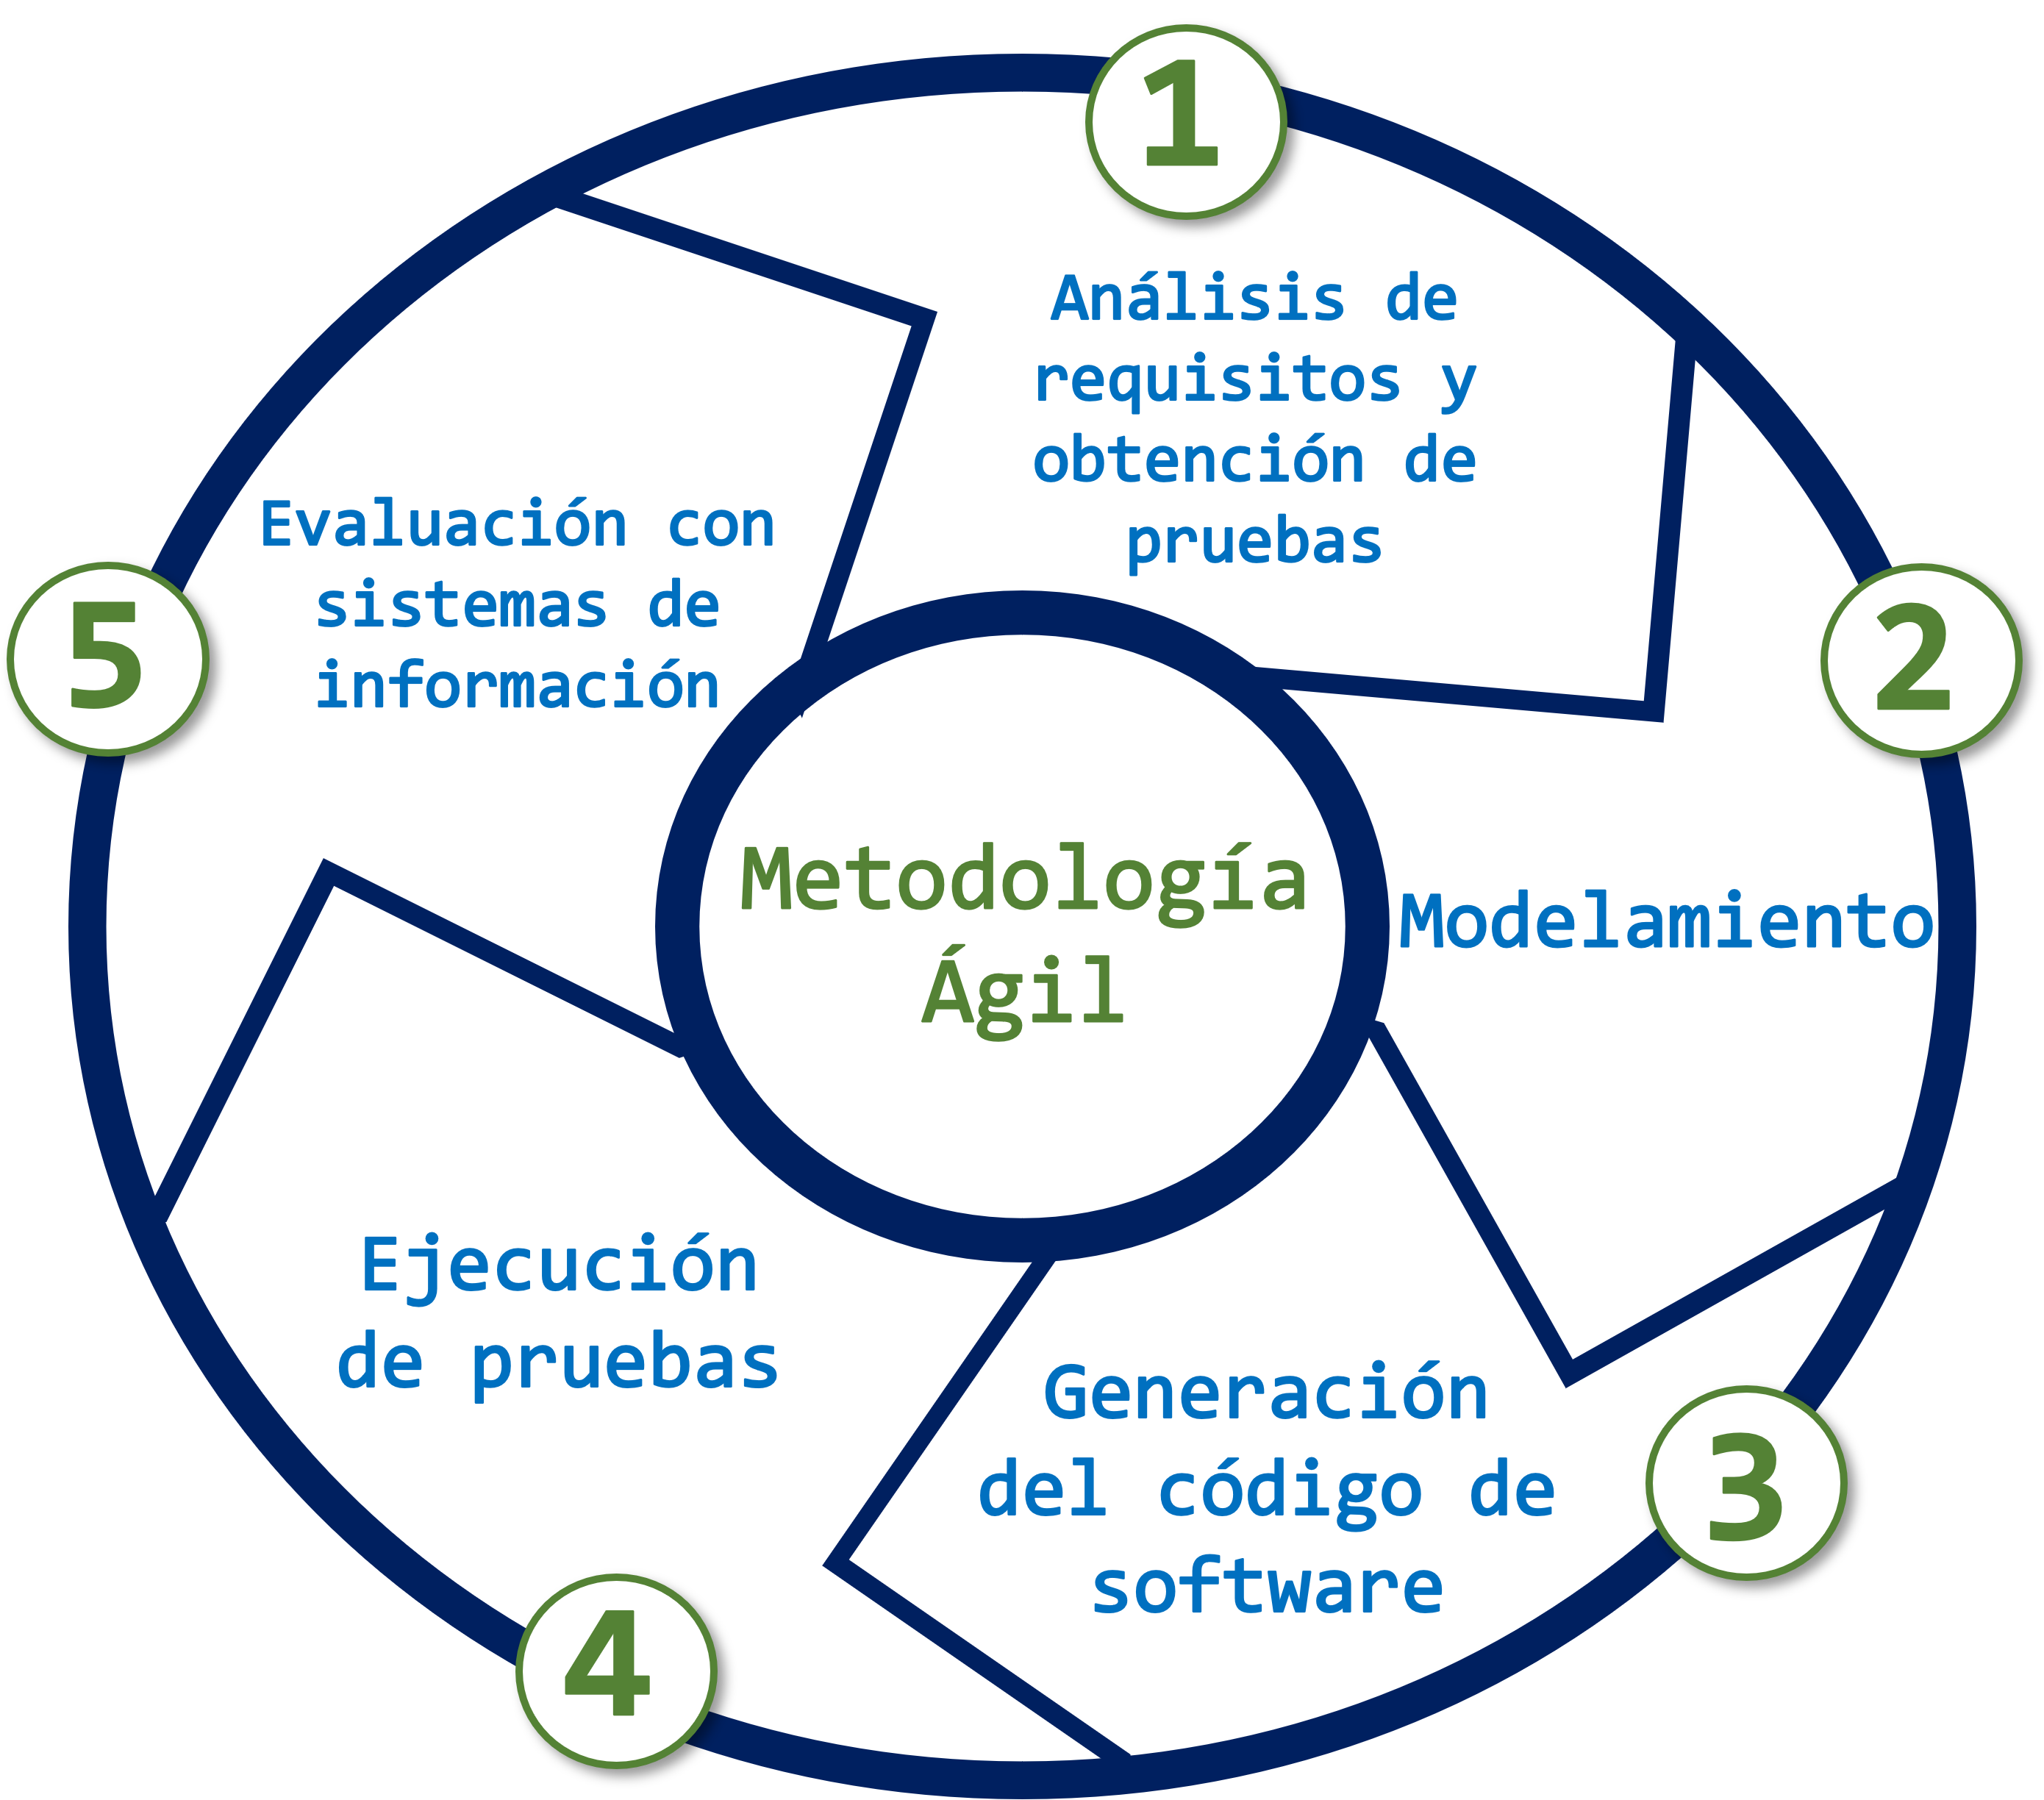
\includegraphics[width=10cm]{img/metodologia.png}
	\label{fig:metod}
	\textbf{\\ ELABORADO: DÚVAL CARVAJAL SUÁREZ}
\end{figure}

Las principales razones del uso de una metodología ágil es el uso de un ciclo de desarrollo iterativo e incremental para la ejecución de este proyecto son:

\begin{itemize}
	\item Entregas frecuentes y continuas de forma que puede disponer de una funcionalidad básica en un tiempo mínimo y a partir de ahí un incremento y mejora continua del sistema.
	
	\item Previsible inestabilidad de requisitos. Es posible que el sistema incorpora más funcionalidades de las inicialmente identificadas
	
	\item Es posible que durante la ejecución del proyecto se altere el orden en el que se desean recibir los módulos.
\end{itemize} 

Para mejorar la ejecución de la metodología se organizaron diferentes tipos de roles que deben ser tomados por las personas que desarrollen del proyecto. Cada rol implementado juega un papel muy importante dentro de la metodología, debido a que deben cumplir tareas de suma importancia para controlar todas las fases que se deben seguir y cumplir los objetivos del trabajo a desarrollar.

\paragraph{Roles}

El equipo de esta metodología está conformado por 2 roles, director de proyecto (DP) y el Desarrollador de Sistemas (DS). Todos los miembros de un equipo de desarrollo tienen diferentes roles en la gestión y supervisión de los proyectos. Todos los roles son necesarios para que el proceso funcione eficientemente.

\begin{itemize}
	\item \textbf{Director de proyecto (DP):} Se encarga de administrar el proceso del proyecto, su planificación, coordinación con el analista y realizar un seguimiento e informes del progreso del proyecto, en términos de calidad, costo y plazos de entrega. El DP es la interfaz principal entre el propietario del producto y el analista de desarrollo de software.
	
	\item \textbf{Desarrollador de Sistemas (DS):} La persona encargada de este rol debe contar con conocimientos de desarrollo de software. El desarrollador deberá estar totalmente familiarizado con el objetivo principal del trabajo. Debido a que será el encargado de analizar todos los requisitos que se necesiten para cumplir con el funcionamiento optimo del sistema, también se encargara analizar, diseñar y codificar el producto final del proyecto.
	
	\begin{itemize}
		\item Comprometerse al inicio de cada módulo y desarrollar todas las funcionalidades en el tiempo determinado.
		
		\item Son responsables de entregar un producto a cada término de un módulo.
		
		\item Definir el desarrollo del sistema.
	\end{itemize} 
\end{itemize}

\paragraph{Fases}

En esta sección se describen cada una de las fases que se mencionaron en el apartado anterior, también se mencionaran breves conceptos relacionados a cada fase y como pueden mitigar los problemas que se pueden presentar a lo largo de la ejecución de la metodología redactada. 

\begin{enumerate}
	\item \textbf{Análisis de requisitos y obtención de pruebas:} Para la recopilación de los requisitos del software es necesario comprenderlos en profundidad para asegurar su correcto funcionamiento cuando este desarrollado. Si al momento de recopilar la información, no lleva todo el tiempo suficiente para ser analizado correctamente podría afectar todo el proyecto en general \cite{Mohamed}.
	
	Para que los requisitos obtenidos sean realizados de manera correcta se pueden priorizar. Existen técnicas actuales para realizar la priorización de requisitos como es el Proceso de Jerarquía Analítica (AHP) ya que produce resultados muy precisos. A continuación se especifican  tres tipos de técnicas de priorización \cite{Mohamed}:
	
	\begin{itemize}
		\item \textit{Escala nominal: } El personal de trabajo que recopilo los requisitos, deberán asignar cada requisito a un grupo de prioridad, transformando a todos los requisitos de ese grupo prioritarios. La asignación numérica, categoriza los requisitos en grupos. Caga grupo cuenta con un identificador único que les permite ser identificados dentro de los demás grupos. 
		\item \textit{Escala ordinal: } Esta técnica produce una lista de requisitos y cada uno cuenta con una prioridad en especifica. Existe una técnica similar a la de escala nominal que se basa en crear varios grupos de prioridad. Pero solo son 3 tipos de grupos: alto, medio y bajo, los desarrolladores priorizan y clasifican los requisitos dentro del mismo grupo en otro subgrupo; ese bucle se repite hasta que cada grupo tenga sólo uno.
		\item \textit{Escala de relación: }Son similares a la escala ordinal, ademas muestran importancia relativa entre todos los requisitos, es decir que dan valores de prioridad a los requisitos.	En estas técnicas, los desarrolladores conocen hasta qué punto cada requisito es más importante que el resto. La votación acumulativa (CV) es una técnica proporcional que depende de la votación de los desarrolladores; cada desarrollador tiene 100 puntos y se distribuyen entre los requisitos en función de su prioridad 
	\end{itemize}
	
	La obtención de pruebas se basa en la recolección de los posibles escenarios que puedan ocurrir al momento consumir el producto final del proyecto. Además, se necesita conocer el resultado que se deberá obtener por los parámetros ingresados por cada prueba. 
	
	\item \textbf{Modelamiento: } El modelado de software básicamente son las abstracciones que describen la arquitectura de un sistema informático. Para llevar a cabo la ejecución de esta fase es necesario tener conocimientos sólidos sobre el desarrollo de software, debido a que los modelos pueden tener diferentes niveles de abstracción y detalles \cite{Kudo}. 
	
	En \cite{Kudo} se propone un metamodelo que permite representar al software a base de patrones de diseño. Es decir, se pueden crear diferentes tipos de diagramas personalizados especificando el comportamiento que tendrá el sistema informático cuando este en ejecución. Además se pueden vincular los patrones encontrados con pruebas de aceptación con los usuarios que usaran el producto final del proyecto presentado. 
	
	\item \textbf{Generación de código:} En la fase de generación de código se relaciona con obtener el producto o software de manera real. En esta etapa los desarrolladores deberán cumplir con algunos puntos claves en el desarrollo de software que son: personalizar la interfaz de usuario, implementar la lógica comercial, integrar servicios de terceros si es necesario o resolver problemas de desarrollo muy complejos que requieran un análisis más profundo para llegar a una solución óptima \cite{Rokis2022}.
	
	Se recomienda a los encargados de ejecutar esta etapa tener conocimientos de programación. En \cite{Rokis2022} mencionan que si la curva de aprendizaje de los desarrolladores es baja, no necesitan obtener conocimientos al momento de generar el código del software. Esto permitirá suponer que el nivel de conocimiento puede impactar en el proceso de aprendizaje y adopción de la tecnología. 
	
	Además para suprimir un poco los grandes desafíos a los que se enfrentan los desarrolladores en este fase, se recomienda el uso de tecnologías con una documentación detallada y cuenten con recursos de aprendizaje. Otra solución potente para ayudar a los desarrolladores es basarse en un sistema similar al que se pretende desarrollar usando el conocimiento de aplicaciones previamente desarrolladas \cite{Rokis2022}.  
	
	\item \textbf{Ejecución de pruebas:} La siguiente fase está relacionada con la primera. Como se podrá observar en los títulos de estas dos fases, se realiza la obtención y ejecución de pruebas sobre el software que se obtendrá. Existen varios problemas que surgen al momento de poner en producción un software desarrollado. En \cite{Gazzola2022} muestran varios estudios que indican que algunos tipos de fallos son intrínsecamente difíciles si no imposibles de detectar en entornos de desarrollo.
	
	Utilizando las pruebas de campo se puede realizar la manipulación del sistema teniendo a la mano los resultados esperados por los datos que son ingresados como entrada sobre el software. Es decir, en esta fase se debe utilizar los datos que fueron recopilados en la primera fase y ser ingresados en el sistema que ya se encuentra totalmente desarrollado. Con el fin de obtener resultados similares o precisamente los mismos a los resultados obtenidos inicialmente \cite{Gazzola2022}.
	
	\item \textbf{Evaluación con sistemas de información:} La fase final de la metodología redactada permitirá usar sistemas de información ya desarrollados que permitan utilizar el producto final del proyecto ejecutado. Se recomienda utilizar sistemas de información con su documentación totalmente detallada, de esa manera se ahorra tiempo en analizar por completo los trabajos para ingresarlos al sistema informático que se desarrolló con esta metodología \cite{Whiting2022}.
	
	
\end{enumerate}

\subsection{Modelo de prototipado}
El Modelo de Prototipado se aplica cuando la información detallada relacionada a requerimientos de entrada y salida del sistema no está disponible. En este modelo se asume que tal vez no todos los requerimientos son conocidos en el inicio del desarrollo del sistema. Se usa generalmente cuando un sistema no existe, o en caso de un largo y complejo sistema, cuando no hay procesos manuales para determinar los requerimientos. Los pasos que se ejecutan en el modelo de prototipado son: 

\begin{enumerate}
	\item \textbf{Obtención y análisis de requisitos:} es el punto de partida del modelo. El usuario es entrevistado para conocer los requisitos del sistema.
	
	\item \textbf{Diseño rápido}: teniendo claro todos los requisitos, se procede a crear un diseño rápido y preliminar incluyendo solo los aspectos más importantes 
	
	\item\textbf{ Construir el prototipo:} se trabaja con la información tomada por el diseño rápido y crear el prototipo de la aplicación.
	
	\item \textbf{Evaluación de usuarios}: el sistema es presentado a varios usuarios para evaluar y verificar sus puntos fuertes y débiles Se reciben comentarios y sugerencias que serán analizadas por los desarrolladores.
	
	\item \textbf{Reajuste del prototipo:} el prototipo actual debe reajustarse según los nuevos requerimientos, es decir que, se debe crear un nuevo prototipo con la información adicional proporcionada por los usuarios evaluados. Este nuevo prototipo será reevaluado justo como el anterior. Este proceso se repite hasta que se cumplan todos los requerimientos especificados por el usuario. Cuando el usuario esté satisfecho con el resultado, se desarrollará un sistema final basado en el prototipo final. 
	
	\item \textbf{Implementación y mantenimiento:} Una vez que se tenga listo el sistema, ya estará listo para ser desplegado a producción. El sistema se somete a un mantenimiento de rutina para minimizar el tiempo de inactividad y evitar fallas a gran escala.
	
\end{enumerate}

\section{Instrumentos de investigación}

\section{Recursos humanos y materiales}

En la siguiente sección se describirán todos los recursos que fueron necesarios para la ejecución del proyecto presentado. Se mencionarán al personal de trabajo que se necesitó y todos los materiales que fueron utilizados. 

\subsection{Talento humano}

Organización y planeación sobre el personal que se encargara de llevar a cabo el proceso de desarrollo del proyecto. Se encarga de coordinar todas las actividades que serán necesarias ser que el proyecto sea culminado con éxito. Además, será el área encarga de definir los tiempos en que se deberá trabajar en todo momento y también designar los tiempos donde se puede descansar para no frutar al personal de trabajo.

\subsection{Equipo de trabajo}

El equipo de trabajo está conformado por una sola persona. Esta persona será la encargada de llevar a cabo la documentación de todo su trabajo realizado, a más de la recopilación de todos los requisitos funcionales y no funcionales para la librería JavaScript. El integrante del equipo es:

\begin{itemize}
	\item Dúval Ricardo Carvajal Suárez
\end{itemize} 

\subsection{Recursos de software}

A continuación se detallaran los recursos de software que fueron necesarios para ejecutar el desarrollo del proyecto presentado:

\begin{table}[h!]
	\caption{Recursos de software utilizados en el proyecto}
	\begin{tabular}{p{3cm}p{6cm}p{5cm}}
		\toprule
		\textbf{Software} & \textbf{Descripción} & \textbf{Vigencia} \\
		\midrule
		Lucidchart & Diseñar algunos gráficos. & Libre (Gratuito) \\
		\addlinespace
		WebStorm & Editor de código para desarrollar la demo de la libreria. & Licencia corporativa (Universitaria) \\
		\addlinespace
		TexStudio & Herramienta para realizar la documentación del proyecto & Libre (Gratuito) \\
		\addlinespace
		Teams & Herramienta para realizar videoconferencias con el tutor de proyecto & Libre (Gratuito) \\
		\addlinespace
		Sistema operativo & Windows 11 & Libre (Gratuito) \\
		\addlinespace
		Programas de oficina & Microsoft Excel, Microsoft Word, Microsoft Power Point & Licencia corporativa (Universitaria) \\
		\addlinespace
		\bottomrule
	\end{tabular}
	
	\textbf{\\ FUENTE: PROPIA \\ ELABORADO: DÚVAL CARVAJAL SUÁREZ}
\end{table}

\subsection{Recursos de hardware}

Los recursos que se observan a continuación son tan necesarios para llevar a cabo la ejecución del proyecto. Como el trabajo se realizó remotamente los recursos físicos corren por cuenta del personal de trabajo.

\begin{table}[h!]
	\caption{Recursos de hardware utilizados en el proyecto}
	\begin{tabular}{p{2cm}p{5cm}p{3cm}p{3cm}}
		\toprule
		\textbf{Cantidad} & \textbf{Equipo} & \textbf{Adquisición} & \textbf{Costo total} \\
		\midrule
		1 & Laptop. & \$ 1.200,00 & \$ 1.200,00  \\
		\addlinespace
		1 & Dispositivo de almacenamiento (Disco duro extraible). & \$ 500,00 & \$ 500,00  \\
		\addlinespace
		\bottomrule
	\end{tabular}

	\textbf{\\ FUENTE: PROPIA \\ ELABORADO: DÚVAL CARVAJAL SUÁREZ}
\end{table}


